% =============================================================
% Discussion and Conclusions -- text of the shared Word version (20 Nov 2026);
% only the corrections are colored (see the legend on page 1).
% =============================================================
\section{Discussion}
\label{sec:discussion}

\subsection{Model performance and generalization}

DINOcow achieved a mean absolute error of 0.415 BCS points on cows never seen during training, with an $R^2$ of 0.72 and a Pearson correlation of 0.85.
This indicates that the model captured a substantial proportion of the variation between cows in body condition while maintaining an error smaller than the 0.5-point interval commonly used in practical BCS assessment.
The close agreement between LOCO validation and repeated five-fold cross-validation, as well as the similar performance of the 12 fully held-out configuration cows, supports the conclusion that the reported accuracy was not inflated by model selection or by repeated exposure to individual animals.

\subsection{Impact of anatomical region selection and feature representation}

A central finding is that anatomical region-based representation substantially improved prediction.
Aggregating frozen DINOv3 features from five \mE{automatically} segmented regions outperformed both whole-image pooling and a single rear-view crop, reducing MAE per cow by 0.081 and 0.111 points, respectively.
This suggests that BCS is not encoded uniformly across the image\mE{, and that} local anatomical cues, particularly those associated with the hook bones, rump and thurl, provide complementary information that is diluted when the model must interpret the entire image.
The absence of additional benefit from including the whole-image descriptor further indicates that background information does not contribute meaningfully to BCS estimation.

Segmenting the cow into six anatomical regions was a useful strategy for improving accuracy and reducing prediction errors.
However, including the \mE{loin} region reduced performance, increasing the MAE per cow from 0.405 to 0.416, and therefore, the final model retained only five regions.
This outcome is plausible because the \mE{loin and its ribs} may be less consistently visible, more affected by posture, lighting, coat pattern, and camera angle, or less directly related to the visual indicators used by trained assessors than the pelvic and tailhead regions\mE{, which indicates} that a more parsimonious anatomical representation can outperform a more complete but noisier one.

The choice of a frozen DINOv3 backbone was also important, as replacing the self-supervised visual features with \mE{hand-crafted} texture descriptors increased MAE per cow from 0.414 to 0.700, while a frozen ResNet-50 representation reached 0.642.
Thus, DINOcow's advantage cannot be attributed solely to anatomical masking or ridge regression\mE{, as} it also reflects the stronger visual representations learned by the foundation model.

\subsection{Comparison of fine-tuned models, identity leakage and data efficiency}

Compared with conventional fine-tuned networks, DINOcow was substantially more accurate on unseen cows.
Fine-tuned ResNet-50, EfficientNet-V2-S, ViT-B/16, EfficientNet-B0, and YOLO classifiers produced \mE{an MAE per cow} between 0.614 and 0.713, or 0.20--0.30 BCS points worse than DINOcow, while their image-level $R^2$ values remained between 0.16 and 0.41.
In contrast, DINOcow reached $R^2 = 0.70$ in the same comparison.
These results show that newer or larger supervised architectures do not necessarily improve BCS prediction when the available \mJ{labeled} dataset is small.

The difference between cow-level and image-level validation is particularly important.
When images from the same cow appeared in both training and test sets, the fine-tuned ResNet-50 and YOLOv8 classifier appeared far more accurate (their MAE fell from 0.656 to 0.232 and from 0.775 to 0.210, respectively).
This improvement reflects identity leakage rather than genuine generalization, because an end-to-end network can memorize the appearance and associated BCS of individual cows.
Under a cow-level split, which \mE{better represents} deployment on new animals entering a herd, DINOcow retained a clear advantage.
Therefore, studies that evaluate BCS models using image-level splits may overestimate \mE{real-world} performance, especially for highly parameterized fine-tuned models.

The proposed approach with segmented regions was also more efficient than fine-tuning the foundation model.
DINOcow fitted only 5.1 thousand coefficients and refit in less than one second on a CPU after feature extraction, whereas DINOv3 with LoRA trained 1.18 million parameters and required approximately 17 minutes of GPU time per fold.
Despite this large difference in training cost, DINOcow was \mE{as accurate as LoRA}, with an MAE per cow of 0.414 versus 0.434\mE{, a difference that was not significant}.
The two methods performed similarly in classifying thin and fat cows, with AUC values of 0.94 and 0.90 for DINOcow \mE{and 0.94 and 0.91 for LoRA}, indicating that the lightweight ridge-based model preserved the practical ability to identify animals at both ends of the condition spectrum.

DINOcow performed well with a small dataset.
Its MAE per cow fell steadily as the number of training cows increased, from 0.69 BCS points with 8 cows to 0.42 with 64, and a fit of the learning curve projected about 0.39 with 100 cows and 0.36 with 200, assuming that new cows resemble the present ones.
Because the error was still decreasing at 64 cows, DINOcow could improve further with a larger and more diverse dataset.
This is especially relevant for precision livestock farming, where collecting large numbers of expert-scored images is expensive and time-consuming.

\subsection{Prediction bias, coat color effects and anatomical discrepancies}

Although the overall bias was only $-$0.02 points, predictions were compressed toward the herd mean, where thin cows were overestimated, and fat cows underestimated.
This regression-to-the-mean behavior is common in supervised regression models and may partly reflect the limited number of extreme BCS observations in the dataset.
The model was most accurate near the middle of the BCS range, where most cows were located, but future work should prioritize balanced sampling of very thin and very fat animals, possibly through targeted data collection or data augmentation.

The observed color-related offset, in which mostly black cows received predictions 0.24 points lower than spotted or piebald cows at the same reference score, is another limitation.
Because only 12 mostly black and 13 mostly white cows were available, this pattern is more likely to reflect underrepresentation than an inherent effect of coat color.
Nevertheless, it highlights the need to evaluate fairness across coat patterns and to include more balanced representation in future datasets.

It is also worth noting that, in some cases, individual body regions did not align with the standard BCS decision tree.
For example, some cows had angular hook bones despite other indicators consistent with a higher score, such as non-visible ribs and non-visible sacral or coccygeal ligaments.
This may reflect non-uniform fat redistribution among body depots, whereby the external appearance of one region does not immediately reflect recent changes in body reserves.
Nevertheless, the available evidence does not establish that some regions change first, or with greater sensitivity, in response to changes in energy balance.
Instead, it indicates that different regions contribute differently to the overall visual perception of BCS and may therefore carry unequal weight in both manual scoring and model-based prediction.

\subsection{Practical application in herd management and industry relevance}

The model achieves applied importance because dietary decisions are influenced by individualized and historical information throughout the lactation period, which is difficult to monitor manually at the individual-cow level.
Around the \mE{weight nadir}, dry matter intake begins to increase, as illustrated in \mR{\mbox{Figure~\ref{fig:lactancia}}}.
This stage can be challenging for ration adjustment because the person responsible for feeding must decide whether to increase ration allocation to promote BCS recovery or maintain the current ration, given that declining milk yield may already reduce the risk of further BCS loss before the next lactation cycle.

\begin{figure}[!htbp]
  \centering
  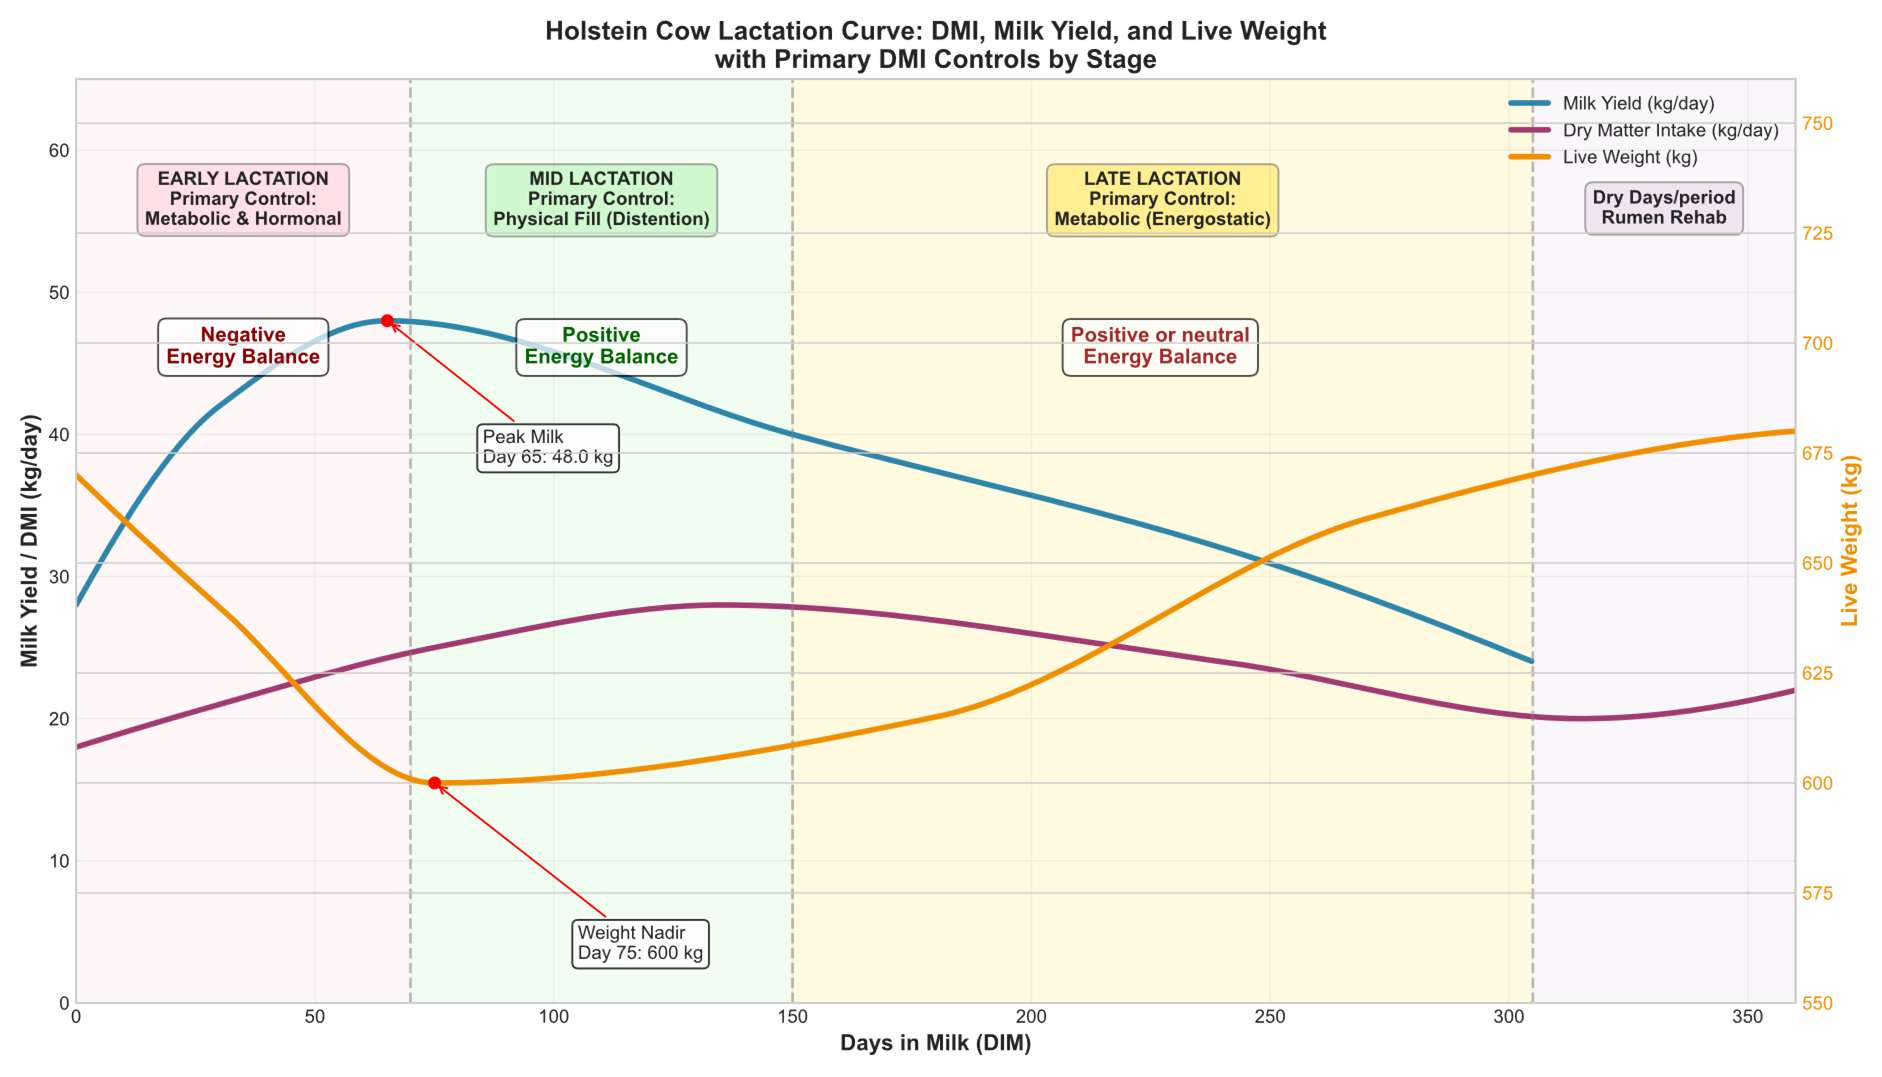
\includegraphics[width=\linewidth]{../figures/word/curva_lactancia.jpg}
  \caption{Representative Holstein cow lactation curve, illustrating the postpartum period around the weight nadir and the subsequent recovery in dry matter intake in relation to the lactation curve.}
  \label{fig:lactancia}
\end{figure}

By providing frequent, cow-specific BCS estimates from routine 2D images, DINOcow could support these decisions by identifying animals whose body reserves are declining, recovering, or remaining stable over time.
This application is supported by the model's day-to-day stability and its ability to follow documented changes in condition, although its value for feeding decisions should be validated against milk yield, DMI, reproductive outcomes, and health records in future studies.
From an industry perspective, the results demonstrate that a 2D-image-based approach can be competitive even though 3D imaging systems often achieve stronger metric performance and are more widely commercialized \mE{\mbox{\citep{mullins2019}}}.
Three-dimensional cameras can capture depth and body-volume information, but they are typically more expensive and may require specialized installation or calibration.

\subsection{Interpretability and regional contributions across lactation}

The relative contribution of each anatomical region to the predicted BCS can be interpreted from how its appearance changes with body condition.
\mE{The hook bones and the right thurl carried the largest contributions at both ends of the scale, whereas the tailhead and the rump moved less} \mR{\mbox{(Figure~\ref{fig:maps})}}.
The thurl is also a practical and validated site for ultrasonographic measurement of backfat thickness, as subcutaneous fat at this site correlates strongly with total body fat and can be compared with BCS \citep{schroder2006}.
\mR{\mbox{Figure~\ref{fig:contrib}} shows} changes in predicted BCS and body-region contribution for four cows with clearly visible changes in BCS\mE{, 2 losing condition in early lactation and 2 gaining it in late lactation}.

\begin{figure}[!htbp]
  \centering
  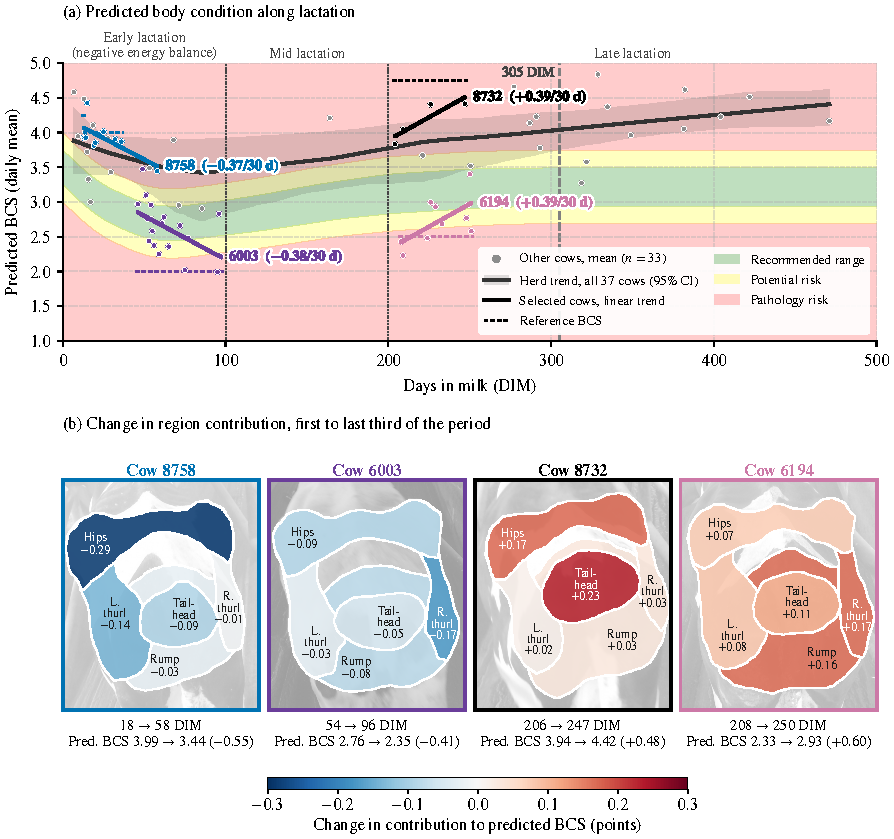
\includegraphics[width=0.97\linewidth]{../figures/bcs_lactation.pdf}
  \caption{Longitudinal changes in predicted body condition and anatomical-region contributions for four cows with clearly visible changes in BCS. (a) Predicted body condition across lactation\mE{ for the 37 cows with known DIM}. (b) Change in relative region contribution from the first to the last third of the observation period.}
  \label{fig:contrib}
\end{figure}

However, these results do not demonstrate that \mE{particular regions change earlier}, or with greater sensitivity, during a shift in energy balance.
Rather, they suggest that visual scorers rely more heavily on these regions when assigning a BCS, and that the model learned a similar regional weighting from the reference scores.

Overall, the findings support anatomically guided transfer learning as a practical strategy for BCS estimation from 2D images.
The combination of region-specific features, a frozen self-supervised backbone, cow-level validation, and a lightweight regression model produced strong generalization to unseen animals while avoiding the computational burden and identity-leakage risks associated with fully fine-tuned deep networks.
Future work should expand the dataset across breeds, parity, lactation stage, coat patterns, farms, and camera conditions, with particular emphasis on thin and fat cows, to test whether the projected improvements in accuracy and bias can be realized in broader commercial settings.

\section{Conclusions}

\begin{marca}{cO}
DINOcow \mE{proved} to be a promising body condition scoring approach for \mE{Holstein dairy cows}, combining anatomical segmentation with frozen self-supervised vision transformer features from conventional 2D rear dorsal images.
The model achieved \mE{an MAE} of 0.405 per cow, with an $R^2$ of 0.72.
\mE{Region-based} descriptions outperformed those derived from the whole image, the cow silhouette, or a single rear crop, indicating that encoding the anatomical areas used in manual assessment yields more informative representations of body condition.
However, the dataset is limited to Holstein cows from CAETEC and a range of BCS 2--5 \mE{in} 0.25 increments.
Overall, frozen foundation model features structured by the \mE{five} regions \mE{used} for scoring offer a practical, data-efficient route to BCS scoring that makes the most out of limited labeled data.
\end{marca}
